\documentclass[a4paper, 14pt]{extarticle}
\usepackage{enumitem}
\usepackage{listings}
\usepackage{xcolor}
\usepackage{graphicx}
\usepackage[justification=centering]{caption}
\usepackage{float}
\usepackage{fefutitle}

\lstdefinestyle{mystyle}{
	basicstyle={\small\ttfamily},
	keywordstyle=\color{orange},
	stringstyle=\color{green},
	basicstyle=\ttfamily\footnotesize,
	breakatwhitespace=false,         
	breaklines=true,                 
	captionpos=b,                    
	keepspaces=true,                 
	numbers=none,                    
	numbersep=5pt,                  
	showspaces=false,                
	showstringspaces=false,
	showtabs=false,                  
	tabsize=2,
	aboveskip=3mm,
	belowskip=3mm,
}
\lstset{style=mystyle}

\begin{document}
	\fefutitle{1}
	\pagebreak	
	\parskip = 5pt

	\section{Задание 1}
		\subsection{Постановка задачи}
			Найти число обусловленности($\mu$) и зависимость $\mu$ от $\mathcal{E}$ системы линейных уравнений: $(A + N \mathcal{E})X = E$, где $A$ -- матрица Гильберта, $N$ -- размерность матрицы, $\mathcal{E} \in [0, 1]$
	
		\subsection{Решение}
		Матрица Гильберта - квадратная матрица с элементами:
		\[ A_{ij} = \dfrac{1}{i + j - 1} \]
		Для нахождения чисел обусловленности напишем программу на Python. Непосредственно вычислением чисел обусловленности будет производить функция cond из библиотеки numpy. Она вычисляет путем умножения второй нормы матрицы на вторую норму обратной матрицы.
		В результате получили следующие значения:

		\begin{enumerate}
			\item $\mathcal{E}  = 0.0, \quad \mu = 16024413500363.82$
			\item $\mathcal{E}  = 0.1, \quad \mu = 89912684538852.02$
			\item $\mathcal{E}  = 0.2, \quad \mu = 168778690000890.22$
			\item $\mathcal{E}  = 0.3, \quad \mu = 247345485434015.62$
			\item $\mathcal{E}  = 0.4, \quad \mu = 326288866751882.1$
			\item $\mathcal{E}  = 0.5, \quad \mu = 406609448878607.1$
			\item $\mathcal{E}  = 0.6, \quad \mu = 484440225993016.06$
			\item $\mathcal{E}  = 0.7, \quad \mu = 565004615280073.2$
			\item $\mathcal{E}  = 0.8, \quad \mu = 641287468678821.8$
			\item $\mathcal{E}  = 0.9, \quad \mu = 721077365256902.4$
			\item $\mathcal{E}  = 1.0, \quad \mu = 801803862815113.0$
		\end{enumerate}
		\begin{figure}[H]
			\centering
			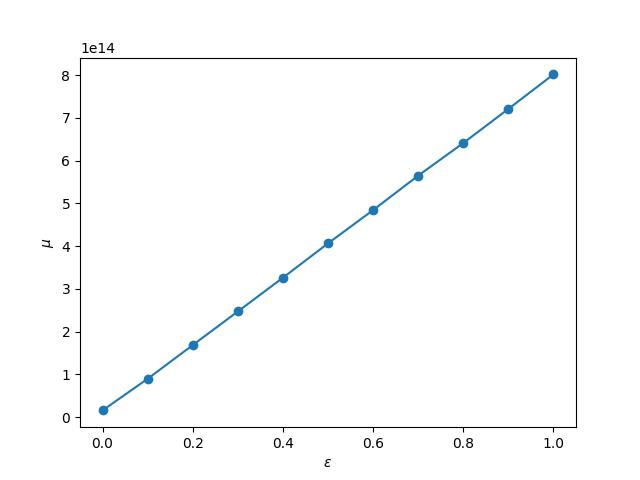
\includegraphics[width = .9\linewidth]{1.jpg}
			\caption[.] {График зависимости $\mu$ от $\mathcal{E}$} 
		\end{figure}
		\pagebreak
		Код программы:
		\begin{lstlisting}[language=Python]
import numpy as np
import matplotlib.pyplot as plt

N = 10
START = 0
END = 1.1
STEP = .1


def build_hilbert_matrix(epsilon):
	hilbert_matrix = [[(1 / (i + j + 1) + N*epsilon) for j in range(N)] for i in range(N)]
	return np.matrix(hilbert_matrix)


def get_conds():
	epsilons = np.arange(START, END, STEP)
	return [np.linalg.cond(build_hilbert_matrix(epsilon)) for epsilon in epsilons]


if __name__ == '__main__':
	epsilons = np.arange(START, END, STEP)
	conds = get_conds()
	print(conds)
	plt.plot(epsilons, conds, marker='o')
	plt.ticklabel_format(useOffset=False)
	plt.xlabel('$\epsilon$')
	plt.ylabel('$\mu$')
	plt.savefig('1.jpg')
		\end{lstlisting}
	
\end{document}	